\documentclass[palatino,nosec]{Docencia}


\title{Cuaderno de clase}
\author{Víctor de Juan}
\date{17/18}

\begin{abstract}
Cuaderno de clase de Matemáticas I, con el desarrollo continuado (sin estar separado por sesiones).
\end{abstract}

% Paquetes adicionales

\usepackage[author={Víctor de Juan, 2017}]{pdfcomment}

\makeatletter
\newcommand{\annotate}[2][]{%
\pdfstringdef\x@title{#1}%
\edef\r{\string\r}%
\pdfstringdef\x@contents{#2}%
\pdfannot
width 2\baselineskip
height 2\baselineskip
depth 0pt
{
/Subtype /Text
/T (\x@title)
/Contents (\x@contents)
}%
}
\makeatother

% --------------------
\newcommand{\cimplies}{\text{\hl{$\implies$}}}
\renewcommand{\vx}{\overset{\rightarrow}{x}}
\renewcommand{\vy}{\overset{\rightarrow}{y}}
\renewcommand{\vz}{\overset{\rightarrow}{z}}
\newcommand{\vi}{\overset{\rightarrow}{i}}
\newcommand{\vj}{\overset{\rightarrow}{j}}
\renewcommand{\vec}[1]{\overset{\rightarrow}{#1}}

\usepackage{pgf,tikz}
\usetikzlibrary{arrows}

\begin{document}
\pagestyle{plain}
\maketitle
\tableofcontents


%% Contenido.

\chapter{Primera evaluación}

\section{Introducción a la asignatura}


Hola, soy Víctor y voy a ser vuestro profesor de matemáticas este año. Algunos me conoceréis, tal vez de campamento o de verme en misa. Para otros tal vez soy totalmente nuevo. ¡Genial! \hl{Soy matemático, entre otras cosas}, y espero poder transmitiros la belleza que encierran las matemáticas.

Reitero que me llamo Víctor y así quiero que me llaméis, ¿bien?

\subsection{Las matemáticas son para siempre}

\href{https://www.ted.com/talks/eduardo_saenz_de_cabezon_math_is_forever}{Vídeo de Eduardo Saenz}

\paragraph{Comentarios al vídeo:}

\begin{itemize}
\item Un teorema es para siempre. ¿Os lo había dicho alguien alguna vez? ¿Qué teoremas conocéis? (Resto, factor, Pitágoras, Tales,  Altura, Euler (V+C=A+2),  ) Pero hay que demostrarlo.
\item Este año está lleno de para siempres. Os voy a enseñar unos buenos teoremas con sus demostraciones a lo largo del curso y vamos a darle importancia a las demostraciones de los contenidos. Cuando la demostración utilice matemáticas que sabéis, las desarrollaremos. 
\subitem \hl{Espero, al final de la clase}, poder enseñaros concretamente a qué me refiero.
\item ¿Alguna pregunta del vídeo? 
\item Weaire-Phelan:
\subitem En la naturaleza, aparece en estructuras químicas (un tipo de cristal).
\subitem \href{https://www.e-architect.co.uk/images/jpgs/beijing/watercube_ptw051208_7.jpg}{El estadio de Pekín de Phelps}
\end{itemize}

\hl{Sed “críticos” en general}. Lo que os cuenten razonadlo. No os lo creáis sin más. Y de esto, nos vamos a hartar en Matemáticas. ¿Alguna pregunta?

\subsubsection{Temario de la asignatura}

El \hl{orden} que vamos a seguir difiere un poco del del libro, porque así nos parece a MariNieves y a mi. 

Vamos a dar un paso más en la resolución de \hl{ecuaciones y sistemas}. 
%
El año pasado resolvíais ecuaciones del tipo: $81^{2x} = \frac{1}{3};\quad x-\sqrt{x-3} = \sqrt{x-2}$, sistemas de ecuaciones 2x2... Este año vamos a ir más allá, vamos a resolver sistemas de 3x3. 

El año pasado tuvisteis una introducción a la geometría. Este año vamos a trabajar con \hl{problemas serios el plano}: distancia punto a recta, distancia entre rectas, cónicas... Por cierto, \ul{¿sabéis porqué se llaman cónicas?}

Y ahora que ya sabéis algo de trigonometría, vamos a ir más allá. Vamos a \hl{exprimir la trigonometría} hasta dominarla. Es algo fundamental en matemáticas. 

Y vamos a dar uno de los temas más bonitos de todo el bachillerato. ¡\hl{Los números complejos}! ¿A alguien le dice algo? ¿A alguien le suena? 
%
Ya veréis que, en realidad, no difíciles. Simplemente arrastramos $\sqrt{-1}$ en las operaciones, como una expresión algebraica, llamando $i=\sqrt{-1}$. 
%
Precioso. 

Y uno de los contenidos centrales del curso, del que hablaréis cuando terminéis el colegio y habréis oído hablar... Las míticas \hl{derivadas}. Os suena, ¿no? 
%
Pues este año nos meteremos en ese berenjenal, a aprender qué es una derivada y para que sirve.
%
También veremos las \hl{Integrales}.
%
Terminaremos el curso con probabilidad y estadística.

Todo esto es una visión general del temario del curso. 
%
Pero hay otro aspecto fundamental de la asignatura. 
%
En otros años lo fundamental puede ser coger habilidad y soltura en los cálculos, saber resolver los problemas... 
%
Este curso va de \hl{razonar y justificar}. Me importa relativamente poco si el resultado está bien o no, en comparación con lo que me importa si el procedimiento está razonado y justificado. 
%
Las matemáticas no son magia, todo tiene una razón de ser. Todo tiene una explicación. 
%
Por ejemplo, ya no nos vamos a centrar tanto en "resuelve esto o lo otro", sino en "demuestra, comprueba, discute esto o lo otro".
%
¿Se entiende?

Por ejemplo, ¿porqué el \hl{teorema de Pitágoras} funciona? 
%
Claro, porque probando con unos números funciona. 
%
¿Quién te asegura que para absolutamente cualquier triángulo rectángulo va a funcionar? Eso hace 4 años te lo creíste. 
%
Este año vamos a demostrar el teorema.

En general, va a haber pocos actos de fe. 
%
En el curso habrá demostraciones y los contenidos no vendrán dados por arte de magia. 
%
Ojo, el teorema fundamental del álgebra no lo podremos demostrar porque hacen falta matemáticas más complejas. 
%
Todo lo demás, lo podremos demostrar.

\subsection{Criterios de evaluación}

Esta asignatura tiene evaluación continua. Eso significa que no hay una recuperación exclusiva para quienes suspendan una evaluación, sino que la primera evaluación es contenido evaluable de la segunda, y la segunda de la tercera.
%
(La primera de la tercera no).

Hay 2 exámenes por evaluación, el primero vale \hl{$\rfrac{1}{3}$} y el segundo \hl{$\rfrac{2}{3}$}. 
%
En ese primer examen, la mitad corresponderá a la evaluación pasada (en caso de que haya evaluación pasada).
%
Si tienes la evaluación suspensa, tienes 5 puntos en el primer examen para recuperar.
%
Si tienes la evaluación aprobada, tienes 5 puntos en el primer examen para repasar.
%
En el segundo examen, en principio, no pondremos contenido de la evaluación anterior.


% -*- root: ../Cuaderno.tex -*-

\chapter{Álgebra}

\section{Repaso de 4º}

\subsection{Logaritmos}

\paragraph{Introducción}

Vamos a aprender una nueva manera de multiplicar. En realidad ya sabéis, aunque no seáis conscientes.\footnote{Fuente: \href{https://www.youtube.com/watch?v=FB3\_BeukBBk\&t=99s}{Mark Foskey, youtube.com}}


\begin{itemize}
\item Caso 1: $1000000·10000000 = 10^6·10^7 = 10^{13}$. ¿Y podremos hacer esto con otros números que no sean el 10?

\item Caso 2: $64·128 = 2^6·2^7 = 2^{13} = 8192$
\item ¿Caso 3?: Me construyo la tabla del 3.
\begin{center}
\begin{tabular}{cccccccccccc}
1& 3& 9& 27& 81& 243& 729& 2187& 6561& 19683& 59049& 177147\\
\textcolor{red}{0} & \textcolor{red}{1} & \textcolor{red}{2} & \textcolor{red}{3} & \textcolor{red}{4} & \textcolor{red}{5} & \textcolor{red}{6} & \textcolor{red}{7} & \textcolor{red}{8} & \textcolor{red}{9} & \textcolor{red}{10} & \textcolor{red}{11}
\end{tabular}
\end{center}
\item Caso 4: ¿Y para números que no son potencias enteras? Por ejemplo, $64*40$. Pues si $32=2^5$ y $64=2^6$, $40=2^{5,...}$ ¿Tiene sentido?

\item Caso 5: Lo que hicieron, Yost y Napier, fue coger la tabla del 1,0001 en lugar de la tabla del 3 y dividir por mil los números rojos, dando lugar a la tabla de logaritmos:

\begin{center}
	\begin{tabular}{cl}
		0.0 & 1.0\\
		0.001 & 1.001\\
		0.002 & 1.002\\
		0.003 & 1.003\\
		0.004 & 1.00401\\
		0.005 & 1.00501\\
		0.006 & 1.00602\\
		0.007 & 1.00702\\
		0.008 & 1.00803\\
		0.009 & 1.00904\\
		$\vdots$ & \quad\quad$\vdots$\\
		0.991 & 2.69259\\
		0.992 & 2.69529\\
		0.993 & 2.69798\\
		0.994 & 2.70068\\
		0.995 & 2.70338\\
		0.996 & 2.70608\\
		0.997 & 2.70879\\
		0.998 & 2.7115\\
		0.999 & 2.71421\\
		1.0 & \hl{2.71692} (Una aproximación de $e$)\\
	\end{tabular}
\end{center}

\end{itemize}

$40=2^{5...}$. Ese $5...$ es lo que llamamos "logaritmo" en base 2 de 40. ¡Los logaritmos son exponentes! Es el \textit{exponente al que hay que elevar} ...


\begin{defn}[Logaritmo]
Sean $a\in ℝ>0,a≠1$ y $N\in\real$.

Se llama logaritmo en base $a$ de $N$ al exponente $x$ que cumple: $a^x = N$ y se escribe:
\[
	\log_aN=x\dimplies a^x=N
\]
\end{defn}

\textbf{Conectando con otras operaciones matemáticas:} 
\[
	\begin{array}{c}
		2^3=8\\
		\sqrt[3]{8}=2\\
		\text{??? }= 3
	\end{array}
\]

La relación $2^3=8$ se puede expresar de otras maneras, dando como resultado el 2 (raíz cúbica) y dando como resultado el 3 (logaritmo).

\nota{De la propia definición se entiende:}
\begin{enumerate}
	\item $y\in\real, y<0 \implies ∀a,\nexists\log_a y$
	\item $\log_a 1 = 0 \dimplies a^0 = 1$
	\item $\log_a a = 1 \dimplies a^1 = a$
	\item $\log_a a^q = q \dimplies a^q = a^q$ por definición.
	\item $a^{\log_a N} = N$
\end{enumerate}

\paragraph{Propiedades}

Vamos a razonar las propiedades de los logaritmos teniendo en cuenta que son exponentes. De hecho, las propiedades de los logaritmos no son otra cosa que las propiedades de las potencias escritas de otra manera.

\begin{itemize}
	\item $\log_a(AB) = \log_a(A) + \log_a(B)$
	\subitem Por ejemplo:
	\[9·8 = 2^x \dimplies x = \log_2 (9·8) = \log_2 8 + \log_2 9\]
	\subitem Como los logaritmos son exponentes, esta propiedad se podría leer: \textit{el exponente de un producto es la suma de los exponentes}.
	\item $\log_a\left(\rfrac{A}{B}\right) = \log_a(A) - \log_a(B)$
	\item Como los logaritmos son exponentes, ¿cómo se leería esta propiedad?
	\item $\log_a(A)^n = n·\log_a(A)$ 

	\item $\displaystyle\log_aA = \frac{\log_bA}{\log_ba}$ \textbf{(Cambio de base})
\end{itemize}

\paragraph{Tomar logaritmos:}

\[
A = B \overset{A>0; a>0; a\neq 1}{\dimplies} a^{\log_a A} = a^{\log_a B} \dimplies \log_aA=\log_aB
\]


\subsubsection{Ejemplos con logaritmos}

Calcula:
\begin{itemize}
	\item $\log \sqrt{0,0001}$
	\item \textit{[Ejercicio de examen de años anteriores]} Demuestra $\log_a b · \log_b a = 1$ 
\end{itemize}


\subsection{Factorización}

\begin{itemize}
	\item Alguien sale a la pizarra a factorizar. Utilizando 
https://www.wolframalpha.com/problem-generator/quiz/?category=Algebra\&topic=FactorPolynomial 
	\item Diferencia raíz y factor.
	\item Verdadero o falso.
	\subitem Un polinomio de grado 2 tiene 2 raíces reales. (Falso: $x^2+1$)
	\subitem Un polinomio con 2 raíces tiene 2 factores. (Discutible: $(x+1)^2(x-1)$)
	\subitem Un polinomio con 2 factores tiene 2 raíces.
	\subitem Un polinomio es irreducible si no tiene raíces reales. (Falso: $P(x) = x^4+2x^2+1$)
	\subitem 2 polinomios con las mismas raíces son iguales: (Falso: $(x^2+1)(x-2)$ y $(x-2)$)
	\subitem 2 polinomios con los mismos factores son iguales: (Falso: $2(x-1)$ y $(x-1)$)

	\item Halla “m” para que $2x^3-2x^2+m·x+4$ sea divisible por $(x-2)$

	\item Deberes: ejercicios 6-9
\end{itemize}


\subsection{Teoremas de factorización}

\paragraph{Ejemplo}
Factoriza: $P(x) = 3x^3-x^2+9x-3 = 3(x^2+3)\left(x-\rfrac{1}{3}\right)$

La factorización del polinomio. ¿Qué raíces puede tener? Ni $\pm1,\pm3$, ¿entonces? Teorema de las raíces racionales.


\hl{\textit{Entregar en hoja aparte: Teoremas de Polinomios}}

\begin{theorem}[Teorema\IS del factor]
Sea $P(x) = a_nx^n+a_{n-1}x^{n-1}+...+a_1x+a_0$ con $a_n≠0$ y $a_n,a_{n-1},...,a_1,a_0\in\real$. 
Sea $α\in\real$.

\[
	P(α) = 0 \dimplies \frac{P(x)}{(x-α)} = Q(x)
\]
\end{theorem}

De hecho este teorema es un caso particular del teorema del resto:
\begin{theorem}[Teorema\IS del resto]
Sea $P(x) = a_nx^n+a_{n-1}x^{n-1}+...+a_1x+a_0$ con $a_n≠0$ y $a_n,a_{n-1},...,a_1,a_0\in\real$.

Entonces, el resto de $\frac{P(x)}{x-α} = P(α)$
\end{theorem}


\begin{theorem}[Teorema\IS de la factorización]
Sea $P(x) = a_nx^n+a_{n-1}x^{n-1}+...+a_1x+a_0$ con $a_n≠0$ y $a_n,a_{n-1},...,a_1,a_0\in\real$ y $α_1,α_2,...,α_n\in\real$ las raíces o ceros de $P(x)$. 

Entonces,\[P(x) = a_n(x-α_1)(x-α_2)...(x-α_n)\]
\end{theorem}


\begin{theorem}[Teorema\IS de las raíces enteras]
Sea $P(x) = a_nx^n+a_{n-1}x^{n-1}+...+a_1x+a_0$, con $a_n≠0$, una raíz entera $r$ de $P(x)$ tiene que ser divisor del término independiente.
\end{theorem}



\begin{theorem}[Teorema\IS de las raíces racionales]
Sea $P(x) = a_nx^n+a_{n-1}x^{n-1}+...+a_1x+a_0$, con $a_n≠0$,$a_i\inℤ$ una raíz fraccionaria $\rfrac{n}{m}$ del polinomio $P(x)$ tiene que cumplir $n|a_0$ y $m|a_n$.
\end{theorem}


\subsubsection{Ejercicios:}

\begin{enumerate}
\item Alguien en la pizarra. Corrijo lo que se haya dejado, escribiendo los teoremas, etc.

Sea $P(x) = 3x^3-3x^2-3x+3$ .¡Factoriza! $P(x) = 3(x-1)(x+1)^2$

\begin{itemize}
	\item ¿Es divisible por $(x-1)$? Comprobamos $P(1) = 3-3-3+3 = 0 \overset{T.F}{\implies}$ Sí.
\end{itemize}

\textit{¡Mira que tontería dice el teorema del factor si miras el polinomio factorizado!}

\item (Ellos) Sea $P(x) = 6x^3-10x^2+4x = 6x(x-1)(x-\rfrac{2}{3})$ 
\begin{itemize}
	\item Factoriza.
	\subitem $P(0) = 0$. Por el teorema del factor sabemos que $x-0$ es un factor.
	\subitem Posibles raíces: $n=\pm1,\pm2,\pm4$ y $m=\pm1,\pm2,\pm3,\pm6$	
	\subitem Por el teorema de la factorización, $Q(x) = 3x^3-5x+2x$ tendrá las mismas raíces que $P(x) = 6x^3-10x^2+4x$. \hl{(Ojo, no podemos simplificar, pero las raíces son las mismas)}. Ahora las posibles raíces son $\rfrac{n}{m}$ donde $n\in\{\pm1,\pm2\}$ y $m\in\{\pm1,\pm3\}$
	\subitem $P(1) = 0$. Por el teorema del factor sabemos que $0$ es una raíz. ¿Es esto más fácil que Ruffini? ¿Y ahora?
\end{itemize}

\item Sea $P(x) = 2x^3-2x^2+kx+4$.
\begin{itemize}
	\item Halla el valor de $k$ para que $P(x)$ sea divisible por $x-2$.
	\subitem Por el teorema del factor, buscamos $P(2) = 0$. Entonces:
	\[
		P(2) = 0 \dimplies 2^4-2^3+2k+4 = 0 \dimplies 16-12+2k = 0 \dimplies k = -2
	\]
\end{itemize}




\item Sea $P(x) = 4x^2+kx+1$.
\begin{itemize}
	\item Halla el valor de $k$ para que sea divisible por $\left(x-\rfrac{1}{3}\right)$. $k=\frac{13}{3}$.
	\item Pero, $3$ no divide a $4$. ¿Cómo podría ser una raíz $\rfrac{1}{3}$?
\end{itemize}


\item Sea $P(x) = 6x^3+ax^2+bx-1$, con $a,b\inℤ$
\begin{itemize}
	\item Halla el valor de $a,b$ para que $P(x)$ sea divisible por $(x-\rfrac{1}{3})$ y por $(x-\rfrac{1}{5})$.
	\subitem Por el teorema de las raíces racionales, $5$ no divide al coeficiente principal, por lo que $P(x)$ no puede ser divisible por $(x-\rfrac{1}{5})$.
	\item Halla el valor de $a,b$ para que $P(x)$ sea divisible por $(x-\rfrac{1}{3})$ y por $(x-\rfrac{1}{2})$.
	\subitem Por el teorema del factor, buscamos:
	\[
	\left\{
		\begin{array}{c}
			P(\rfrac{1}{2}) = 0 \dimplies \frac{6}{8} + \frac{a}{4} + \frac{b}{2} - 1 = 0\\
			P(\rfrac{1}{3}) = 0 \dimplies \frac{6}{27} + \frac{a}{9} + \frac{b}{3} - 1 = 0
		\end{array}\right\}\dimplies ... \quad (a,b) = (-1,-4)
	\]
\end{itemize}

\item\textbf{Ampliación, puesto pero sin corregir} Sea $P(x) = 4x^2+bx+1$, con $b∈ℤ$. 
\begin{itemize}
	\item Sabemos que sus raíces $α_1,α_2$ son fraccionarias y negativas. ¿Cuáles son? ¿Cuánto vale $b$?
	\subitem Por el teorema de las raíces racionales, $α_1 = \rfrac{n_1}{m_1}$, sabemos que $n_1$ divide a $1$. Análogo para $α_2$.

	Por otro lado, sabemos que $m_2$ divide a 4. Las posibilidades son $2,4$, con lo que $α_1,α_2 \in \{\rfrac{1}{2},\rfrac{1}{4}\}$

	Por el teorema del factor, $P(\rfrac{1}{2}) = 1+b\rfrac{1}{2}+1 = 0 \implies b=-4$. 

	Por el teorema del factor, $P(\rfrac{1}{4}) = \rfrac{1}{4}+b\rfrac{1}{4}+1 = 0 \implies b=-2$.

	Si queremos que sea divisible por los 2 factores, b tiene que valer a la vez $4$ y $-2$. Entonces, necesariamente $P(x) = 4(x-\rfrac{1}{2})^2$ o $P(x) = 4(x-\rfrac{1}{4})^2$. 

	Desarrollando la segunda opción, obtenemos como término independiente $\rfrac{1}{4}≠1$, por lo que no es posible. 
	%
	Por otro lado, desarrollando la primera opción obtenemos algo con sentido.

	\[
		4\left(x+\rfrac{1}{2}\right)^2 = 4\left(x^2+x+\rfrac{1}{4}\right) = 4x^2+4x+1 \implies b=4
	\]

\end{itemize}

	\item Factorizar $P(x) = 9x^3-\frac{27}{2}x^2+\frac{13}{2}x-1 = 9·(x-1/2)(x-2/3)(x-1/3)$. Pista (para ahorraros pruebas innecesarias con Ruffini), todas las raíces son fraccionarias y positivas.

	\item Factorizar $P(x) = x^7+2x^4+x = x(x^3+1)^2$

	

\item Sea $P(x) = 21x^2+10x-2$. $P(x) + 3 = 21(x+1/3)(x+1/7)$.

\end{enumerate}




\section{Tema 2: Ecuaciones}

\subsection{Teoría sobre ecuaciones}


\begin{example}
\[
	-20 = -20 \dimplies 25-45 = 16-36 \dimplies 5^2-5·9 = 4^2-4·9 \dimplies 5^2-5·9+\left(\rfrac{9}{2}\right)^2 = 4^2-4·9+\left(\rfrac{9}{2}\right)^2 \dimplies
\]
\[
	\left(5-\rfrac{9}{2}\right)^2 = \left(4-\rfrac{9}{2}\right)^2 \text{\hl{\;\;;\;\;}} 5-\rfrac{9}{2} = 4-\rfrac{9}{2} \dimplies 5=4
\]
\end{example}


\obs Dividir por 0 no mantiene la equivalencia.
%
En general, tomar una raíz no mantiene equivalencia entre ecuaciones (tampoco elevar a una potencia).

\begin{defn}[Ecuaciones equivalentes]
Dos ecuaciones son equivalentes si tienen las mismas incógnitas y las mismas soluciones.
\end{defn}

\paragraph{Clasificación de ecuaciones}

Las ecuaciones según sus soluciones pueden ser:
\begin{itemize}
	\item Incompatible: no tiene ninguna solución. Ejemplo: $5x=5x+2$
	\item Compatible determinada: tiene un número finito de soluciones. Ejemplo: $3x=6$.
	\item Compatible indeterminada: tiene infinitas soluciones. Ejemplo $2x-\frac{3x-1}{3} = x+\frac{1}{3}$. Solución: $x=λ, ∀λ∈ℝ$.
\end{itemize}


\begin{example}
	¿Son equivalentes?
	\begin{itemize}
		\item $9x=3x^2 \dimplies 9=3x$ [CD]
		\item $9=3x \dimplies x=3$ [CD]
		\item $4=5 \dimplies 1=0$ [IN]
		\item $9x=3^2x \dimplies 0x=0$ [CI]
		\item[difícil] $9x=\frac{(3x)^2}{x} \dimplies 9x=9x$ [CI]

\paragraph{Conclusiones:} \textbf{¡Ojo con simplificar ecuaciones!} Cuando "desaparezcan" incógnitas mirar con cuidado, porque estaremos perdiendo soluciones en la inmensa mayoría de los casos.

¿Cuándo no?

	\item $\frac{\sqrt{9x^2}}{x^2}=\frac{3x}{x^2} \dimplies \frac{9}{x} = \frac{9}{x} \dimplies 0=0$
	\end{itemize}
\end{example}



\subsection{Racionales}

Ecuaciones racionales.

\paragraph{Ejemplo}
\[
	\frac{2x}{x-2} + \frac{3x}{x+2} = \frac{7x^2}{x^2-4} \dimplies \frac{2x(x+2)}{(x-2)(x+2)} + \frac{3x(x-2)}{(x+2)(x-2)} = \frac{7x^2}{x^2-4} \dimplies 
\]
\[
	\frac{2x(x+2)+3x(x-2)}{x^2-4} = \frac{7x^2}{x^2-4} \text{\hl{$\implies$}} 2x^2+4x+3x^2-6x=7x^2 \dimplies 5x^2-7x^2-2x = 0 \dimplies 
\]
\[
	x(-x-1) = 0 \dimplies x_1 = 0 \wedge x_2 = -1
\]

\hl{¿Son soluciones las 2?}

La equivalencia la hemos perdido si $x\neq \pm2$, por lo que las soluciones $x_1 = 0 \wedge x_2 = -1$ son válidas (\ul{y no es necesario hacer la comprobación}).



\hl{Ejercicios: 84 ad + propios con trampa de equivalencias}


\paragraph{Cuidado:} casuística nueva de equivalencias e implicaciones. Hasta ahora, los valores peculiares de las implicaciones que no son equivalencias sólo nos ahorraban alguna comprobación\footnote{que tampoco está demás hacer para asegurarnos que hemos operado bien}.
%
Pero puede darse el caso de que pasen otras cosas. Por ejemplo, ¿qué pasa en esta simplificación?

\[(x-1)·\frac{x}{x+1} = (x-1)·(x^2-9) \text{\hl{$\implies$}} \frac{x}{x+1} = x^2-9\]

A la izquierda el 1 es solución y a la derecha no, luego las ecuaciones no son equivalentes. Pero, ¿qué pasa con el $x=1$?

En esta implicación he \ul{perdido una solución}. Es una equivalencia si $x\neq 1$, y en el caso $x=1$, tengo una solución. 

\paragraph{Más ejemplos}
\begin{itemize}
	\item
	\[
		\frac{1}{1-\frac{1}{x+1}} = \frac{x+1}{x} \dimplies \frac{1}{\frac{x+1-1}{x+1}}=\frac{x+1}{x} \dimplies \frac{x+1}{x} = \frac{x+1}{x} \text{\hl{$\implies$}} x=λ, ∀λ∈ℝ\setminus\{0,-1\}
	\]

	\item
	\[
		\frac{1+\displaystyle\frac{x+1}{x-1}}{2-\displaystyle\frac{x-1}{x+1}}=2 \dimplies \frac{\displaystyle\frac{x-1+x+1}{x-1}}{\displaystyle\frac{2x+2-x+1}{x+1}} = 2 \dimplies
	\]
	\[	
		\frac{\displaystyle\frac{2x}{x-1}}{\displaystyle\frac{x+3}{x+1}}=2 \text{\hl{$\implies$}} 2x^2+2x=x^2+4x-6 \dimplies 2x=6 \dimplies x=3
	\]

	\item

	\[
		\frac{3}{x} - \frac{x}{x+2} = \frac{5x-1}{x^2+x-2}
	\]

	\item Ejercicios 83 y siguientes del libro.
\end{itemize}

\subsection{Ecuaciones irrracionales}

\paragraph{Ejemplo:}
\[
	\sqrt{x+1} - \sqrt{x^2-5}=0 \text{\hl{$\implies$}} x+1 = x^2-5 \dimplies (x_0,x_1) = (3,-2)
\]

\textbf{Comprobamos} porque hemos perdido la equivalencia: 

$\sqrt{-2+1} = \sqrt{(-2)^2-5} \dimplies \sqrt{-1} = \sqrt{-1}$; -2 no es una solución en los reales.

Por otro lado: $\sqrt{3+1} = \sqrt{3^2-5} \dimplies \sqrt{2}=\sqrt{2}$

\textit{La comprobación no sería necesaria si hubiéramos reparado en que la equivalencia se mantendría siempre que el interior de las raíces fuera positivo, es decir $x\geq -1 \wedge x\geq \sqrt{5}$}

\paragraph{Ejercicio:} 
\[
	\sqrt{x+4}+\sqrt{x-1} = 5 \text{\hl{$\implies$}} (x+4)+(x-1) + 2\sqrt{(x+4)(x-1)} = 25 \text{\hl{$\implies$}} (22-2x)^2 = 4(x^2+3x-4) \dimplies 
\]
\[
	4x^2-88x + 484 = 4x^2+12x-16 \dimplies -100x + 500 = 0 \dimplies x=5
\]

Comprobamos:
\[
	\sqrt{5+4}+\sqrt{5-1} = 3+2 = 5
\]

\textit{Aquí la comprobación si resulta mucho más útil porque nos ahorra resolver la inecuación $(x+4)(x-1) \geq 0$}

\begin{itemize}
	\item Dudas.
	\item Corregir irracional. 89b.
	\item 85e,90a no lo hagáis.
	\item Empezamos 
\end{itemize}



\subsection{Exponenciales y logarítmicas}

Pregunta: $a^x=a^y \overset{?}{\dimplies} x=y$

$x=y\implies a^x=a^y$ Sí.

$a^x=a^y\implies x=y$ No. Contraejemplo: $1^2=1^3$.  Basicamente, si los logaritmos no mantenían la equivalencia, tampoco lo iban a hacer estas.

Siempre que la base no sea $0,±1$ sí serán equivalentes. ¿Y si tenemos un polinomio como base? Pues como puede ser uno de esos valores, no mantenemos la equivalencia o calculamos para qué valores sí sería equivalente o no.

Trabajamos 108abc, 109ac,111c (el más difícil de todos)

\subsection{Logarítmicas}

Los logaritmos tampoco conservan las equivalencias:

Versión innecesariamente larga:
\[
	-5 = -5 \dimplies -30+25 = 1-6 \dimplies -30+25+9 = 9+1-6 \dimplies (3-5)^2 = (3-1)^2 \dimplies 
\]
\[
	\log(3-5)^2 = \log(3-1)^2 \dimplies 2\log(3-5) = 2\log(3-1) \dimplies \log(3-5)=\log(3-1) \dimplies \log2=\log-2
\]

Versión corta:
\[
	(-2)^2 = (2)^2 \text{\hl{$\implies$}} 2\log(-2) = 2\log(2) \dimplies \log(-2) = \log(2) \dimplies -2=2
\]

Ecuación de ejemplo:


\[
	\log x=t \implies 5t=3t+\log6^2 \dimplies 2t=2\log6 \dimplies t=\log6 \dimplies \log x=\log6 \text{\hl{$\implies$}} x=6
\]

Si estás más versado en la abstracción algebraica:

\[
	5\log x=3\log x+2\log 6 \dimplies 2\log x=2\log6 \text{\hl{$\implies$}} x=6
\]


Incluso, habría una tercera manera:
 
\[
	5\log x=3\log x+2\log 6 \dimplies \log x^5=\log36x^3 \dimplies x^5=36x^3 \dimplies
\]
\[
	x^5-36x^3 = 0 \dimplies x^3(x^2-36) = 0 \dimplies x^3(x+6)(x-6) = 0
\]




\paragraph{Ejercicio}
\[
	\log\frac{2x-2}{x} = 2\log(x-1)-\log x \dimplies \log \frac{2x-2}{x}=\log\frac{(x-1)^2}{x} \cimplies \frac{2(x-1)}{x} = \frac{(x-1)^2}{x} \overset{1}{\cimplies}
	\]
	\[ 
	x-1=2 \dimplies x=3
\]
En 1 hemos simplificado 2 factores. $x$ y $(x-1)$. En esta simplificación podríamos haber perdido soluciones, en concreto, si $0,1$ fueran soluciones no lo obtendríamos. 

En este caso no son solución porque $\log 0$ no existe.

\paragraph{Ejercicio}
\[
\frac{\log (4-x)}{\log(x+2)}=2 \cimplies \log(4-x) = \log(x+2)^2 \cimplies 4-x=(x+2)^2 \dimplies 4-x=x^2+4x+4 \dimplies
	\]
	\[ x^2+5x=0 \dimplies x_1=0 \wedge x_2=-5
\]
$x_2=-5$ no es solución porque $\nexists\log(-5+2)=\log(-3)$. Por otro lado, $\frac{\log4}{\log2} = \log_24=2$ cqc.



\paragraph{Ejercicio} mientras corrigen

\[
	\log_x 3 = \ln \sqrt{3} \dimplies \frac{\ln3}{\ln x}=\ln\sqrt{3} \dimplies \frac{\ln3}{\ln x}=\frac{\ln3}{2} \dimplies \frac{1}{\ln x}=\frac{1}{2} \implies \ln x = 2 \implies e^2=x
\]

\paragraph{Ejercicio}
\[
	\log_332+\log_{\rfrac{1}{3}}(6-x) = \log_{\sqrt{3}}x \dimplies \log_332+\frac{\log_3(6-x)}{\log_3\rfrac{1}{3}} = \frac{\log_3x}{\log_3{\sqrt{3}}} \dimplies 
\]
\[
	\log_332-\log(6-x)=2\log_3x\dimplies \log_3\left(\frac{32}{6-x}\right)=\log_3x^2 \cimplies 32=x^2(6-x) \dimplies -x^3+6x^2-32 = 0
\]
\[
	-(-2)^3 + 6(-2)^2-32 = 8+24-32 = 0\implies x_1=-2 \wedge x_2=x_3=4
\]
 
Comprobamos:

\[
	\log_332+\log_{\rfrac{1}{3}}(6-4) = \log_{\sqrt{3}}4 \dimplies \log_332-\log_32=\log_34^2 \dimplies \log_3\frac{32}{2}=\log_316 \;\;\text{   cqc.}
\]



\section{Sistemas de ecuaciones}

Minimísimo repaso a la reducción como método para resolver sistemas de ecuaciones.

\subsection{Sistemas lineales: Gauss}

Por grupos, resolver:
\[
\left\{\begin{array}{lccccc}
e_1: &2x&+y&-2z&=&7\\
e_2: &x&+y&+z&=&0\\
e_3: &3x&+2y&+2z&=&1
\end{array}\right\} \dimplies (x,y,z) = (1,1,-2)
\]



Clase 1: Explicación de los apuntes de MariNieves y realización de 1 sistema.

Clase 2: Realización de un ejemplo por mi parte. Tiempo de trabajo para ellos.

Clase 3 (11/10/2017): Corrección ejercicio del libro + dudas del examen. 

\paragraph{Sesión 17/10:} Examen.

\paragraph{Sesión 18/10:} Sistemas de Gauss C.Indeterminados e Incompatibles.

\paragraph{Sesión 19/10:} 
\begin{itemize}
	\item Corregimos (si quieren) 113 incompatible y CI.
	\item ¿En qué consiste discutir un sistema? Escribir completo los 3 casos
	\item Sistemas con parámetros
\end{itemize}

\paragraph{Discusión de un sistema}

Una vez llegado al \hl{sistema escalonado} pueden darse 3 situaciones:

\begin{itemize}
	\item La ecuación con una única incógnita es incompatible $\implies$ Sistema Incompatible.
	\item Número de incógnitas > número de ecuaciones $\implies$ Compatible indeterminado.
	\item Número de incógnitas = número de ecuaciones, siendo la última ecuación compatible determinada $\implies$ Compatible determinado.
\end{itemize}


\subsection{Sistemas no lineales}

Ejercicios: 114cf (f es interesante),115acdf

\[
\left\{
	\begin{array}{c}
		x^2-2xy+y^2 = 1\\
		x^2-y^2 = 12\\
	\end{array}
\right\}
\]

\chapter{Geometría}

\section{Vectores en $\real^2$}

\begin{defn}[Vector fijo]
Segmento orientado.
\end{defn}

\obs Un segmento orientado tiene un principio, un final, una dirección, un sentido y una longitud (o módulo).

Por ejemplo, el vector que une $(1,3)$ con $(2,2)$. Pero estos vectores necesitan un hábitat. ¿Dónde viven? En el conjunto de los puntos. 

¿Existe el punto $(e,π)$? Claro que sí. De una manera general, el conjunto de los puntos son pares de números reales. La manera formal y matemática de definir el conjunto de puntos es el producto cartesiano.

\begin{defn}[Producto cartesiano]
Sean $A$ y $B$ 2 conjuntos. Se define el producto cartesiano como

\[
	A\times B = \left\{ (a,b) \tq a\in A \wedge b\in B \right\}
\]
\end{defn}

\obs $A\times B \neq B\times A$

\begin{example}
\[\{2,4,6\}\times \{1,3,5\} = \{(2,1),(2,3),(2,5),(4,1),...,(6,5)\}\]
\[\{1,3,5\}\times \{2,4,6\} = \{(1,2),(1,4),(1,6),(3,2),...,(6,5)\}\]
\end{example}

Vamos a \hl{definir $\real^2$}, con el que vamos a trabajar a partir de ahora. 

\[\real^2 = \real\times\real = \{ (x,y)\in\real^2 \tq x,y\in\real\}\]

\begin{example}
	\begin{itemize}
		\item $(2,3)\in\real^2$
		\item $(\sqrt{-1},\pi)\not\in\real^2$
		\item $(e,\sqrt{2})\in\real^2$
	\end{itemize}
\end{example}


\subparagraph{Representación de estos elementos en el plano}

\textit{Dibujo del plano y representación de los ejemplos. ¿Puntos?¿Vectores?}
De momento puntos, porque para poder tener vectores necesitamos tener un origen, un destino, una longitud, una dirección y un sentido. ¿No?

No, ¿verdad? Los vectores del año pasado no nos importaba el origen ni el destino. Sólo nos importaban módulo, dirección y sentido. ¿Por qué? Porque trabajábamos con vectores libres. ¿Qué es un vector libre?

\paragraph*{Vectores libres}

\begin{defn}[Vector libre]
Representante canónico del conjunto de vectores con mismo módulo, dirección y sentido.
\end{defn}

Como las fracciones equivalentes. $[\rfrac{1}{2}] = \{\rfrac{1}{2},\rfrac{2}{4},\rfrac{4}{8},...\}$. Distintas maneras de expresar la misma realidad.



$\real^2$ por si sólo no es nada, asique vamos a definir operaciones en esta estructura algebraica.



\subsection{Operaciones en $\real^2$}
\subsubsection{Suma:}
$\appl{+}{\real^2\times\real^2}{\real^2}$  y se define como $(a,b)+(c,d) = (a+c,b+d)$.

\begin{example}
$(2,3) + (-1,4) \overset{(1)}{=} (2+(-1),3+4)  \overset{(2)}{=} (1,7)$

Donde en $(1)$ aplicamos la suma en $\real^2$ y en $(2)$ aplicamos la suma en $\real$.

\hl{\textbf{Representación gráfica de la suma}} (en dibujos sin base. Sobre fondo liso.)

\end{example}

\subparagraph{Propiedades de la suma en $\real^2$:} Formalmente, \textit{ley de composición interna.}

\begin{itemize}
	\item \textbf{Conmutativa: } $(a,b)+(c,d) = (c,d)+(a,b), \;\forall (a,b),(c,d)\in\real^2$
	\item \textbf{Asociativa: } $\left((a,b)+(c,d)\right) + (e,f) = (a,b)+\left((c,d)+(e,f)\right), \;\forall (a,b),(c,d),(e,f)\in\real^2$
	\item \textbf{Elemento neutro: } $(a,b) + (0,0) = (a,b), \;\forall (a,b)\in\real^2$.
	\item \textbf{Elemento simétrico: } $(a,b) + (-a,-b) = (0,0) \;\forall (a,b)\in\real^2$
\end{itemize}

\obs El par $(\real^2,+)$ es un grupo conmutativo.

\subsubsection{Producto por un escalar} Formalmente, \textit{ley de composición externa con con dominio de operadores en $\real$.}

$\appl{·}{\real\times\real^2}{\real^2}$ y se define como $λ·(a,b) = (λa,λb), \;\forallλ\in\real,(a,b)\in\real^2$

\begin{example}
$2·(\sqrt{2},\pi) = (2\sqrt{2},2\pi)$

\hl{\textbf{Representación gráfica}} (en dibujos sin base. Sobre fondo liso.)

\end{example}

\subparagraph{Propiedades del producto con dominio de operadores en $\real$}

\begin{itemize}
	\item \textbf{Distributiva} para los escalares: $(α+λ)·(a,b) = α(a,b) + λ(a,b), \;\forall α,λ\in\real,\;\forall(a,b)\in\real^2$
	\item \textbf{Distributiva} para los elementos de $\real^2$: $λ·\left((a,b)+(c,d)\right) = λ(a,b) + λ(c,d), \;\forall λ\in\real,\;\forall(a,b),(a,b)\in\real^2$
	\item \textbf{Asociativa para los escalares: } $λ·(α·(a,b)) = (λ·α)(a,b), \;\forallλ,α\in\real,\;\forall(a,b)\in\real^2$
	\item \textbf{Elemento neutro} $1·(a,b) = (a,b), \;\forall(a,b)\in\real^2$ 	
\end{itemize}


¿Podemos decir que $\real^2$ es un cuerpo? Para ello tendríamos que definir $(a,b)·(c,d),\;\forall(a,b),(c,d)\in\real^2$, cosa que no hemos hecho. A la estructura algebraica $(\real^2,+,·)$ tal y como la hemos definido la llamamos \concept[Espacio\IS Vectorial]{Espacio vectorial}.

Igual que hemos definido $\real^2$, podríamos haber definido $\real^3$, estructura con la que trabajaréis el año que viene. De hecho, podríamos definir $\real^{25}$ de una manera muy similar.
%
Como curiosidad matemática, hasta podríamos definir $\real\times...\times\real$ infinitas veces y estudiar qué pasa con ello. 

¿Y todo esto en qué se concreta? Vamos a aterrizar toda esta abstracción matemática. Los elementos de $\real^2$ no son otra cosa que los vectores con los que trabajábamos el año pasado.

\subsubsection{Combinaciones lineales}

\begin{defn}[Combinación lineal]
Combinación lineal de $\vec{x},\vec{y},\vec{z}\in\real^2$ es cualquier expresión algebraica de la forma $α\vec{x}+β\vec{y}+λ\vec{z}$ con $α,β,λ\in\real$
\end{defn}

\begin{example}
	\begin{itemize}
		\item $2·(1,1) + \sqrt{2}·(0,1) = (2,2+\sqrt{2})$
		\item $1·(1,0) + (-\rfrac{1}{2})(2,0) = (0,0)$ (\textit{Combinación lineal nula})
		\item Venga, ponedme 2 ejemplos vosotros.
	\end{itemize}
\end{example}

\begin{defn}[Dependencia lineal]
Sean $\vec{x},\vec{y},\vec{z}\in\real^2$. 

\[\vz \text{ depende linealmente de } \vx,\vy \dimplies \existsα,λ\in\real \tq \vz = α\vx+λ\vy\]
\end{defn}

También podríamos definirlo para 2 vectores. $α·\vx = λ·\vy$.

¿Existen $α,β\in\real$ para que $α(1,0) = λ(0,1)$? No. Bueno, $α=λ=0$.

\begin{defn}[Independencia lineal]
Sean $\vec{x},\vec{y}\in\real^2$. 

\[\vx,\vy \text{ linealmente independientes } \dimplies \left(α\vx+λ\vy = (0,0) \implies α=λ=0\right)\]
\end{defn}

\begin{problem} Demostrar que $a=(2,2)$ y $b=(3,5)$ son linealmente independientes.
\solution

Buscamos $α,β$ tales que $αa+βb = (0,0)$. 

\[
	α(2,2) + β(3,5) = (0,0) \dimplies (2α+3β,2α+5β) = (0,0) \dimplies 
\]
\[
\left\{
	\begin{array}{c}
		2α+3β = 0\\
		2α+5β=0
	\end{array}
\right\}\dimplies 
\left\{
	\begin{array}{c}
		2α+3β = 0\\
		2β=0
	\end{array}
\right\}\dimplies (α,β) = (0,0) 
\]
\end{problem}

\begin{problem} Halla el valor o valores de $m$ para que  $a=(1,3)$ y $b=(2,m)$ sean linealmente dependientes.
\solution

Por definición de dependencia lineal, buscamos $α,β$ tales que $αa+βb = (0,0)$.

\[
α(1,3) + β(2,m) = (0,0) \dimplies (α+2β,3α+m·β) = (0,0) \dimplies 
\]
\[
\left\{
	\begin{array}{c}
		α+2β = 0\\
		3α+m·β=0
	\end{array}
\right\}\overset{(1)}{\dimplies}
\left\{
	\begin{array}{c}
		α+2β = 0\\
		(m-6)β=0
	\end{array}
\right\}
\]
\textit{donde $(1): E_2=E_2-3E_1$}

Si $m=6$, tenemos $0β=0$, cuya solución es $β\in\real$. 

\textbf{Conclusión:} para $m=6$ los vectores son linealmente dependientes. Valdría tomar $β=-1$ y $α=2$.

Comprobación: $αa+βb = 2(1,3)+(-1)(2,6) = (2-2,6-6) = (0,0)$
\end{problem}

\obs $(1,3),(2,6)$ son linealmente dependientes porque son proporcionales. Esto es cierto en general:

\begin{prop}
Los vectores $\vx=(x_1,x_2),\vy=(y_1,y_2)\in\real^2$ son linealmente dependientes $\dimplies \frac{x_1}{y_1}=\frac{x_2}{y_2} \text{ (es decir, son proporcionales)}$ 
\end{prop}


\begin{problem} Halla el valor o valores de $m$ para que  $a=(1,3)$ y $b=(2,m)$ sean linealmente dependientes.
\solution

Utilizamos: "2 vectores son linealmente dependientes si y sólo si son proporcionales".

Buscamos $m$ tal que $\rfrac{1}{2} = \rfrac{3}{m}$, lo cual es cierto si $m=6$.
\end{problem}

\begin{defn}[Rango de un conjunto de vectores]
El rango de un conjunto de vectores es el número de vectores linealmente independientes que contiene.
\end{defn}

\begin{example}
	\begin{itemize}
		\item $\text{Rg}\{(0,1),(1,0),(0,3)\} = 2$
	\end{itemize}
\end{example}

\begin{problem}
Halla los valores de $m$ para los que el conjunto de vectores $C=\{(1,3),(3,m)\}$ tenga rango 2. ¿Hay algún valor para que el rango sea 0?

\solution

\end{problem}

\section{Plano afín}

\paragraph{Concreción de lo abstracto} 

¿Qué necesitamos para orientarnos en el plano? ¿Cuál puede ser un sistema de referencia? No copiar, primero entender.\textit{Con la pizarra borrada, sitúo un punto. ¿Cómo ponernos de acuerdo para definirle unas coordenadas? Necesitamos un origen y una base}


Sistema de referencia: un origen y una escala (base). Normalmente tomamos como origen el $(0,0)$ y como base la canónica $\{(1,0),(0,1)\}$.

\subsubsection{Base de un espacio vectorial}

\begin{defn}[Sistema de generadores]
$B = \{\vx_1,\vx_2,...,\vx_n\}$ con $\forall i=1,...,n\;\;\vx_i,\in\real^2$ es un sistema de generadores si y sólo si $\forall \vz\in\real^2,\;\; \existsα_1,α_2,...,α_n\in\real \tq \vz=α_1\vx_1+α_2\vx_2 + ... + α_n\vx_n \left( = \sum_{i=1}^n α_i\vx_i\right)$
\end{defn}

\begin{defn}[Base]
Un conjunto $B=\{\vx,\vy\}$ con $\vx,\vy\in\real^2$ es una base de $\real^2$ si y sólo si cumple:

	\begin{itemize}
		\item $\vx,\vy$ linealmente independientes.
		\item $\{\vx,\vy\}$ es un sistema de generadores.
	\end{itemize}

\end{defn}

\begin{example}
	\begin{itemize}
		\item Sea $B_1=\{(0,1),(1,0)\}$ una base de $\real^2$. El vector $(3,6)$ tiene de \concept[Coordenadas de un vector]{coordenadas} $3$ y $6$ porque $(3,6) = 3·(1,0) + 6·(0,1)$.
		\obs $B_1$ se denomina base canónica y se suele representar por $B=\{\vi,\vj\}$.

		\item ¿Es una base?
			\begin{problem}
			\ppart ¿Es $B_2 = \{(1,1),(1,-1)\}$ una base de $\real^2$?
			\ppart ¿Cuáles son las coordenadas del vector $(7,5)$ en esta base?

			\solution
			\spart Buscamos demostrar que los vectores son linealmente independientes y que las coordenadas de un vector cualquiera $\vz=(z_1,z_2)$ son únicas. 

			\paragraph{Independencia lineal:} 

			\[
				(0,0) = α(1,1) + β(1,-1) \dimplies (0,0) = (α+β,α-β) \dimplies 
			\]
			\[
				\left\{
					\begin{array}{c}
						α+β=0\\
						α-β=0
					\end{array}
				\right\}\dimplies
				\left\{
					\begin{array}{c}
						α+β=0\\
						2α=0
					\end{array}
				\right\}\implies (α,β) = (0,0)
			\]

			\paragraph{Generación:} Las coordenadas de un vector cualquiera $\vz=(z_1,z_2)$ deberían ser únicas.

			\[
				(z_1,z_2) = α(1,1) + β(1,-1) \dimplies (z_1,z_2) = (α+β,α-β) \dimplies 
			\]
			\[
				\left\{
					\begin{array}{c}
						α+β=z_1\\
						α-β=z_2
					\end{array}
				\right\}\dimplies
				\left\{
					\begin{array}{c}
						α+β=z_1\\
						2α=z_2
					\end{array}
				\right\}\dimplies (α,β) = (z_1-\rfrac{z_2}{2},\rfrac{z_2}{2})
			\]

			Dado un vector cualquiera hemos encontrado una expresión única de sus coordenadas. 
			%
			Entonces, el conjunto genera $\real^2$.

			\spart 
			\[
				(7,5) = α(1,1) + β(1,-1) \dimplies (7,5) = (α+β,α-β) \dimplies 
			\]
			\[
				\left\{
					\begin{array}{c}
						α+β=7\\
						α-β=5
					\end{array}
				\right\}\dimplies
				\left\{
					\begin{array}{c}
						α+β=7\\
						2α=12
					\end{array}
				\right\}\implies (α,β) = (6,1)
			\]
			\end{problem}

	\end{itemize}
\end{example}



\begin{figure}[h]
\centering
\definecolor{xdxdff}{rgb}{0.49,0.49,1}
\definecolor{ttqqff}{rgb}{0.2,0,1}
\begin{tikzpicture}[line cap=round,line join=round,>=triangle 45,x=1.0cm,y=1.0cm]
\draw[->,color=black] (-1.8,0) -- (4.14,0);
\foreach \x in {-1,1,2,3,4}
\draw[shift={(\x,0)},color=black] (0pt,2pt) -- (0pt,-2pt) node[below] {\footnotesize $\x$};
\draw[color=black] (4.04,0.02) node [anchor=south west] { x};
\draw[->,color=black] (0,-0.33) -- (0,3.31);
\foreach \y in {,1,2,3}
\draw[shift={(0,\y)},color=black] (2pt,0pt) -- (-2pt,0pt) node[left] {\footnotesize $\y$};
\draw[color=black] (0.03,3.19) node [anchor=west] { y};
\draw[color=black] (0pt,-10pt) node[right] {\footnotesize $0$};
\clip(-1.8,-0.33) rectangle (4.14,3.31);
\draw [->,line width=1pt] (0,0) -- (1,0);
\draw [->,line width=1pt] (0,0) -- (0,1);
\draw [->,line width=1pt,color=ttqqff] (0,0) -- (1,0.5);
\draw [->] (0,0) -- (1,2);
\draw [->,line width=1pt,color=ttqqff] (0,0) -- (-0.2,1);
\draw [->] (0,0) -- (-0.27,1.36);
\draw [->] (0,0) -- (1.27,0.64);
\draw [dotted,domain=-1.8:4.14] plot(\x,{(-1.91--1.36*\x)/-0.27});
\draw [dotted,domain=-1.8:4.14] plot(\x,{(--1.91--0.64*\x)/1.27});
\begin{scriptsize}
\draw[color=black] (0.47,-0.1) node {$i$};
\draw[color=black] (-0.06,0.48) node {$j$};
\draw[color=ttqqff] (0.56,0.21) node {$v$};
\fill [color=xdxdff] (0,0) circle (1.5pt);
\draw[color=xdxdff] (0.05,0.08) node {$A$};
\draw[color=ttqqff] (-0.13,0.41) node {$u$};
\draw[color=black] (-0.21,1.15) node {αu};
\draw[color=black] (1.12,0.61) node {βv};
\draw[color=black] (-1.75,0.73) node {$c$};
\end{scriptsize}
\end{tikzpicture}
\caption{Cambio de base de otros vectores que no tienen nada que ver, hecho gráficamente .}
\end{figure}

\paragraph{Ejercicio}
\begin{problem}
Sea $B=\{(3,0),(1,-1)\}$. 
\ppart ¿Es una base de $\real^2$?
\ppart En caso de que sea una base, calcula las coordenadas del vector $(6,6)$ en la base $B$.
\ppart ¿Es una base ortogonal?
\solution
\spart
\textbf{Linealmente independientes:}
\[
α(3,0) + β(1,-1) = (0,0) \dimplies \left\{\begin{array}{c}3α+β=0\\-β=0 \end{array}\right\} \dimplies  (α,β) = (0,0)
\]
\textbf{Generadores:} 
\[
α(3,0) + β(1,-1) = (x,y) \dimplies\underbrace{\left\{\begin{array}{c}3α+β=x\\-β=y \end{array}\right\}}_{SCD} \dimplies  (α,β) = (\rfrac{x+y}{3},-y) \implies \exists! (a,b)\in\real^2
\]

\spart 
\[
	(6,6) = α(3,0) + β(1,-1) \dimplies (6,6) = (3α+β,-β) \dimplies (α,β) = (4,-6)
\]
\end{problem}


\subsection{Repaso:}

\subparagraph{Coordenadas de un vector entre los puntos $A=(a_1,a_2)$ y $B=(b_1,b_2)$:} 

$[\vec{OA}] + [\vec{AB}] =  [\vec{OB}] \dimplies [\vec{AB}] =  [\vec{OB}] - [\vec{OA}] = (b_1,b_2) - (a_1,a_2) = (b_1-a_1,b_2-a_2)$


\subparagraph{Vector de posición} Llamamos $[\vec{OA}]$ al vector de posición del punto $A=(a_1,a_2)$, cuyas coordenadas son $[\vec{OA}] = (a_1-0,a_2-0)=(a_1-a_2)$


\begin{example}
Hallar las coordenadas de $[\vec{AB}]$ con $A=(1,2)$ y $B=(3,5)$.

$[\vec{AB}] = (1-3,2-5)$
\end{example}

\begin{problem}
Sean 3 puntos $A=(1,-1), B=(0,2), C=(-1,m)$.

\ppart Halla, si es posible, el valor de $m$ para que $[\vec{AB}] = [\vec{BC}]$

\ppart Halla, si es posible, el valor de $m$ para que $[\vec{AB}] = [\vec{AC}]$

\solution

\spart 
\[
\left.\begin{array}{l}
	[\vec{AB}] = (-1,3)\\
	\left[\vec{BC}\right] = (-1,m-2)
\end{array}\right\} \implies m-2=3 \dimplies m=5
\]

\spart 
\[
\left.\begin{array}{l}
	[\vec{AB}] = (-1,3)\\
	\left[\vec{AC}\right] = (-2,m+1)
\end{array}\right\} \implies \text{ Imposible } [\vec{AB}] = [\vec{AC}]
\]


\end{problem}

\subparagraph{Punto medio de un vector} \textit{Apoyarse en un dibujo} $A=(a_1,a_2)$ y $B=(b_1,b_2)$. 

Por definición, el punto medio $M=(m_1,m_2)$ cumplirá: $[\vec{AM}] = [\vec{MB}]$

\[
[\vec{AB}] = [\vec{AM}] + [\vec{MB}]
[\vec{AB}] = 2[\vec{AM}] \dimplies 
2(m_1-a_1,m_2-a_2) = (b_1-a_1,b_2-a_1) \dimplies
\]
\[
\left\{
	\begin{array}{c}
	2m_1-2a_1 = b_1-a_1\\
	2m_2-2a_2 = b_2-a_2
	\end{array}
\right\}\dimplies
\left\{
	\begin{array}{c}
	m_1 = \displaystyle\frac{b_1+a_1}{2}\\
	m_2 = \displaystyle\frac{b_2+a_2}{2}
	\end{array}
\right\}
\dimplies (m_1,m_2) = \left(\frac{b_1+a_1}{2},\frac{b_2+a_2}{2}\right)
\]


\paragraph{Módulo de un vector:} Sea $\vec{x} = (x_1,x_2)$. ¿Cuál es la longitud del vector en la base canónica? (\textit{Dibujar.} Pitágoras.)

$\norm{\vec{x}} = \sqrt{x_1^2+x_2^2}$

¿Y si fuera otra base? ¿Se mantendría? No

\subsection{Producto escalar}

\begin{defn}[Producto escalar]
Sean $\vx=(x_1,x_2),\vy=(y_1,y_2)\in\real^2$. 

El producto escalar es una operación: $\appl{·}{\real^2\times\real^2}{\real}$ que opera de la siguiente manera: 

\[\vx·\vy = |\vx|·|\vy|·\cos{\hat{(\vx,\vy)}}\]
\end{defn}

\paragraph{Propiedades:} $\forall\vx,\vx,\vz\in\real^f2$

\begin{itemize}
	\item \textbf{Conmutativo: } $\vx·\vy = \vy·\vx$
	\item \textbf{Bilineal:}
	\subitem  $(λ\vx)·\vy=λ(\vx·\vy)$
	\subitem  $\vx·(\vy+\vz) = \vx·\vy + \vx·\vz$
	\item \textbf{No negatividad:} $\vx·\vx ≥0$
\end{itemize}


\begin{defn}[Ortogonalidad]
$\vx,\vy\in\real^2$ son ortogonales $\dimplies \vx·\vy=0$.
\end{defn}

\begin{defn}[Perpendicular]
$\vx,\vy\in\real^2$ son perpendiculares $\dimplies$ forman un ángulo recto.
\end{defn}

¿Es lo mismo perpendicular que ortogonal? Perpendicular $\implies$ ortogonal, pero no al revés.

\begin{defn}[Norma de un vector]
	$\norm{\vx} = \vx·\vx$
\end{defn}


\subsection{Ejercicios}


\begin{problem}
Sea $B=\{(-2,2),(1,-1)\}$. 
\ppart ¿Es una base de $\real^2$?
\ppart En caso de que sea una base, calcula las coordenadas del vector $(6,6)$ en la base $B$.
\solution
\spart
\textbf{Linealmente independientes:}
\[
α(-2,2) + β(1,-1) = (0,0) \dimplies \left\{\begin{array}{c}-2α+β=0\\2α-β=0 \end{array}\right\} \dimplies \underbrace{\left\{\begin{array}{c}-2α+β=0\end{array}\right\} }_{SCI}
\]
Los vectores no son linealmente independientes. Tomando $α=1,β=2$ por ejemplo.

\textbf{Generadores:} 
Ni me lo planteo.


\spart 
Menos todavía.

\end{problem}

\begin{problem}
Sean $A=(0,0),B=(-1,3),C=(2,5)$. ¿Están alineados?
\solution

Que estén alineados es lo mismo que decir que 2 de ellos sean linealmente dependientes, o proporcionales y que tengan algún punto en común.

$[\vec{AB}] = (-1,3)$, $[\vec{AC}] = (2,5)$. Como vectores fijos tienen en común el punto $A$. ¿Son L.D.? 

\[
	\frac{-1}{2} ≠ \frac{3}{5} \implies \text{ No L.D.} \dimplies \text{ No alineados.}
\]

\end{problem}

\begin{problem}
Sean $A=(0,0),B=(-1,3),C=(m,m+8)$. Halla $m$ para que estén alineados.
\solution
$[\vec{AB}] = (-1,3)$, $[\vec{AC}] = (m,m+8)$

\[
	\frac{-1}{m} = \frac{3}{m+8} \implies -m-8 = 3m \dimplies -8=4m \dimplies m=-2
\]

\obs También podríamos haber construido el vector $[\vec{BC}]$, pero hemos elegido $[\vec{AC}]$ por simplificar los cálculos.
\end{problem}

\begin{problem}
Sean $A=(0,0),B=(-1,3),C=(2,m)$. Halla $m$ para que $|[\vec{AB}]| = λ|[\vec{AC}]|$
\solution

$[\vec{AB}] = (-1,2\sqrt{6}) \to |[\vec{AB}]| = \sqrt{1+24}=5$

$[\vec{AC}] = (3,m) \to |[\vec{AB}]| = \sqrt{9+m^2}$

Necesitamos $\sqrt{9+m^2} = 5 \implies 9+m^2 = 25 \dimplies m^2=16 \dimplies m=\pm4$.

\end{problem}

\section{Geometría Analítica}

Ha sido muy caótico...


\subsection{Lugares geométricos}

Definición, fórmula, desarrollo fórmula (por el libro), ejemplo.

\begin{itemize}
	\item Circunferencia.
	\subitem Posición relativa de recta y circunferencia. Intersección y distancia.
	\subitem Halla $k$ para que la recta $Ax+By+k=0$ sea tangente a la circunferencia.
	\item Mediatriz.
	\subitem 2 maneras de calcular. Ejercicio 53 (ellos).
	\item Bisectriz. 
	\subitem Ejercicio 55 (yo).
	\subitem Ejercicio 56 (ellos).
	\subitem Deberes: 127.
	\subitem Lugar geométrico de los puntos del plano que equidistan de 2 rectas paralelas.
	\item Elipse: suma de distancias a los focos.
	\subitem Fórmula (deducción del libro), eje mayor, eje menor.
	\subitem Focos eje $X$, focos eje $Y$.
	\subitem Deducir la fórmula dado un dibujo.
	\subitem Ejercicio 18.
	\subitem Si $a<b$, la ecuación $\rfrac{x^2}{a} + \rfrac{y^2}{b} = 1$ representa una elipse cuyo eje mayor está contenido en el eje Y.
	\item Hipérbola: diferencia de distancias a los focos.
	\subitem Fórmula, eje mayor, eje menor.
	\subitem Focos eje $X$, focos eje $Y$.
	\subitem Forma ejercicio 22.
	\subitem Actividad resuelta 161.34.
	\item Parábola: equidista foco y directriz.
	\subitem Ejercicio resuelto 24 (yo). ¿Cuántas soluciones?
	\subitem Parábola de directriz x=3. ¿Forma?
	\subitem El punto medio entre la directriz y el foco siempre pertenece a la parábola. ¿V/F?
\end{itemize}


\begin{itemize}
	\item Trabajo cooperativo. 
	\item Los 3 lugares geométricos que faltan. Imponer la restricción de distancias en los 3. Ver en el libro la deducción de las fórmulas y a lo que llegamos.
	\item Ejercicio 18.
	\item Ejercicio 22 cambiando enunciado (forma de la hipérbola).
	\item Ejercicio 25 cambiando enunciado (forma de la parábola).
	\item Sin geogebra:
		\subitem Esboza la hipérbola 59ad parábolas del 62abhi.
	\item Con geogebra: 
		\subitem 55d (salvo excentricidad). ¿Qué pasa si intercambias el 6 y el 10? 
		\subitem 59a (salvo excentricidad). ¿Qué pasa si intercambias el 144 y el 25?

\end{itemize}

\subsubsection{Cónicas}
A saber:
\begin{itemize}
	\item Reconocer y diferenciar los 4 tipos de cónicas, tanto gráfica como algebraicamente.
	\item Conocer la definición como lugar geométrico de los puntos de los 3 tipos de cónicas.
	\subitem Aplicar la definición para contestar cuestiones breves.
	\item Dibujar a mano alzada una cónica dados los datos necesarios (una directriz y un foco, etc).
	\item Resolver posición relativa de una recta y una cónica (resolver el sistema).
	\item Halla $k$ para que la recta $Ax+By+k=0$ sea tangente a la circunferencia.

\end{itemize}

\chapter{Trigonometría}

Sentarles por parejas.

\section{Repaso de 4º}

¿Qué es un radián? Pequeño debate sobre una medida de ángulos que no dependa de una medida externa (como podría ser una circunferencia).

Geogebra del radián (ver \ref{img:radian}). Trabajar el concepto de radián y la equivalencia. ¿Hablas inglés pensando en español o en inglés? Este año toca \textit{pensar en radianes}.

\begin{figure}
\centering
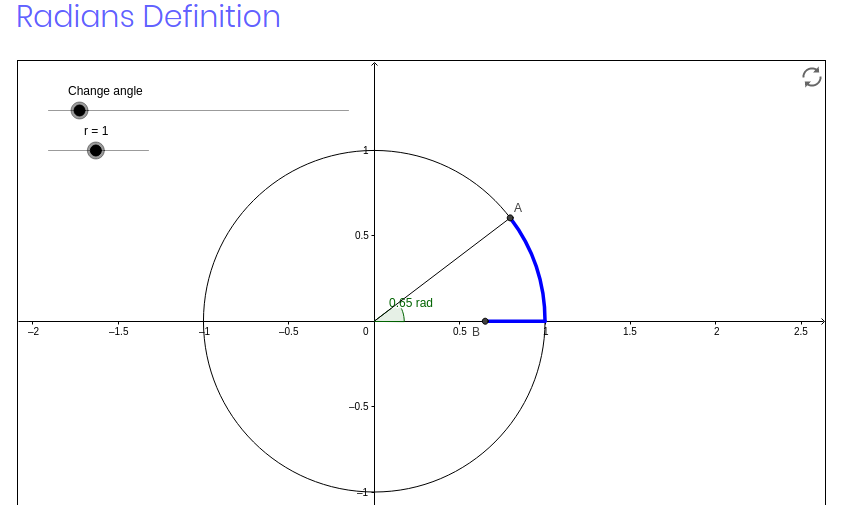
\includegraphics[scale=0.5]{img/Trigon1}
\caption{Definición de radián}
\label{img:radian}
\end{figure}

Utilizando geogebra (ver \ref{img:razones}) las razones trigonométricas en la circunferencia goniométrica. 
\begin{itemize}
	\item ¿De dónde vienen los nombres? 
	\item ¿Triángulos rectángulos para aplicar Pitágoras?
\end{itemize}

\begin{figure}
\centering
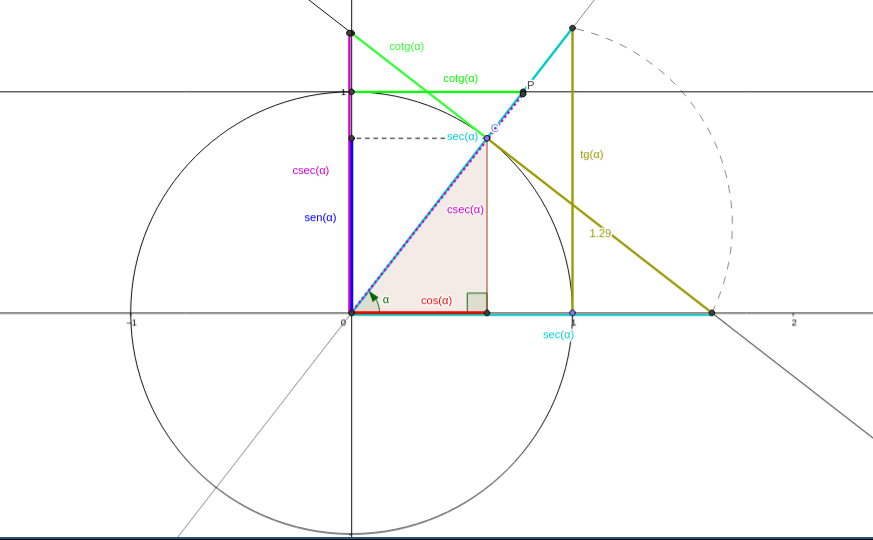
\includegraphics[scale=0.5]{img/Trigon2}
\caption{Razones trigonométricas}
\label{img:razones}
\end{figure}


Proyectando el libro, explicar:
\begin{itemize}
	\item Identidades trigonométricas (página 80). Ojo al "ten en cuenta de la izquierda".
	\item Signo de las razones trigonométricas (página 77).
	\item Reducción al primer cuadrante (página 78).
	\item Tabla de valores notables.
	\item Ángulos complementarios.
\end{itemize}

Ejercicios 16 del libro (utilizando las 2 páginas donde vienen todas las fórmulas) [Corregimos proyectando el libro].

Demuestra (corregimos proyectando el libro). 
\[
	\frac{\cosα-\secα}{\senα-\cosecα} = \tg^3α
\]

Deberes: demuestra algebraicamente $\tg^2α+1=\sec^2α$ y $\cotg^2α+1=\cosec^2α$

\section{Identidades trigonométricas}

\subsection{Suma y diferencia de ángulos}

\begin{figure}[hbtp]
\centering
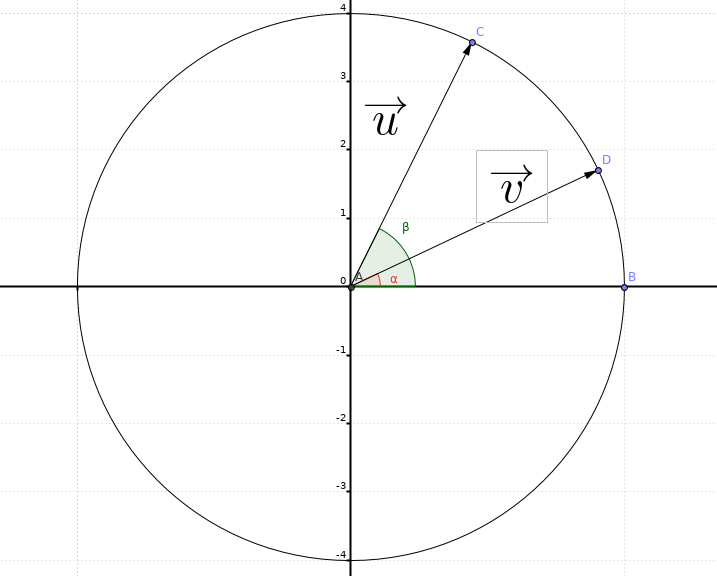
\includegraphics[scale=0.5]{img/Trigon3}
\caption{Razonamiento coseno de la diferencia.}
\label{img:cosenodif}
\end{figure}


Las coordenadas de $\vec{u} = (\cosβ,\senβ)$ y $\vec{v} = (\cosα,\senα)$. Vamos a calcular $\vec{u}·\vec{v}$, teniendo en cuenta que son vectores unitarios.

\[
	\vec{u} · \vec{v} = |\vec{u}| · |\vec{v}| · \cos(β-α) \dimplies (\cosβ,\senβ)·(\cosα,\senα) = \cos(β-α)
\]
\[
	\cos(β-α) = \cosβ\cosα - \senβ\senα
\]
Escribiendo $α=-α$, obtendríamos las razones del ángulo suma.

\begin{example}
	\begin{itemize}
		\item $\sen\left(\rfrac{5π}{12}\right) = \sen\left(\rfrac{2π}{12} + \rfrac{3π}{12}\right)$
	\end{itemize}
\end{example}

Para trabajar (ellos):
\begin{itemize}
		\item $\cos\left(\rfrac{π}{2}+\rfrac{π}{3}\right)$ (ellos)
		\item $\sen\left(\rfrac{π}{12}\right)$ (ellos)
		\item Demuestra: $\displaystyle \tgα+\tgβ = \frac{\sen(α+β)}{\cosα\cosβ}$
\end{itemize}

\subsubsection{Ángulo doble y ángulo mitad}

\begin{itemize}
	\item $\cos(2α)$ (ellos)
	\item $\sen(2α)$ (ellos)
	\item Calcula $\cos\left(\rfrac{α}{2}\right)$ utilizando $\sen^2β+\cos^2β=1$ y $β=\rfrac{α}{2}$
	\item $\sen\left(\rfrac{β}{2}\right)$
\end{itemize}

Fin clase 2.

\section{Resolución de triángulos}

\chapter{Números complejos}

\section{Introducción} 
Vamos a interntar resolver $x^2 + 9 = 0 \dimplies x^2 = -9 \dimplies x=\sqrt{-9}$. Siempre hemos dicho que no tiene solución. Pero yo podría escribir $(\sqrt{-9})^2 + 9 = 0$. Es decir, $\sqrt{-9}$ es solución de la ecuación. ¡Y también lo es $x_2=-\sqrt{-9}$!

La manera de trabajar con raíces negativas es sacar todos los factores hasta dejar simplemente $\sqrt{-1}$, es decir: $\sqrt{-9} = \sqrt{9}\sqrt{-1} = \pm3\sqrt{-1}$ y escribimos $\sqrt{-1} = i$. \textbf{Conclusión:} las soluciones de la ecuación son $x_1 = 3i$ y $x_2 = -3i$.

Pongamos otro ejemplo:


¿Podríamos factorizar el polinomio $P(x) = x^2-2x+2$? El \textbf{teorema fundamental del álgebra} dice que tiene 2 soluciones, pero las 2 son complejas. Vamos a verlo

Para factorizar el polinomio calculamos sus raíces resolviendo la ecuación: $P(x) = 0$

\[x^2-2x+2 = 0 \dimplies x=\frac{2\pm\sqrt{4-4·1·2}}{2} = \frac{2\pm\sqrt{-4}}{2} = \frac{2}{2} \pm \frac{2i}{2} = 1\pm i\]

Hemos obtenido 2 raíces: $α_1 = 1+i$ y $α_2 = 1-i$. ¿Cómo quedaría el polinomio factorizado? \[P(x) = x^2-2x+2 = (x-α_1)·(x-α_2) = (x-(1+i))·(x-(1-i))\]

Primera utilidad de los números complejos: resolver ecuaciones que antes eran "imposibles" y factorizar polinomios que considerábamos irreducibles.


\section{Operaciones en $ℂ$}

Un número complejo es de la forma $z=a+bi$, donde $i=\sqrt{-1}$, y llamamos $a=Re(z)$ y $b=Im(z)$. 

\paragraph{Ejemplos}
\begin{itemize}
	\item $z_1 = 3$ $\to$ $Re(z_1) = \;\;\quad\quad\;\;\;$; $Im(z_1) = \;\;\;\;\;\;\;$ \footnote{Luego, todos los números reales son complejos.}
	\item $z_2 = 2-i$ $\to$ $Re(z_2) = \;\;\quad\quad\;\;\;$; $Im(z_2) = \;\;\;\;\;\;\;$
	\item $z_3 = \sqrt{2}+6i$ $\to$ $Re(z_3) = \;\;\quad\quad\;\;\;$; $Im(z_3) = \;\;\;\;\;\;\;$
	\item $z_4 = i^4$ $\to$ $Re(z_4) = \;\;\quad\quad\;\;\;$; $Im(z_4) = \;\;\;\;\;\;\;$
\end{itemize}

\paragraph{Representación gráfica:} como los vectores en física, sólo que aquí no hay $\vec{i}$ ni $\vec{j}$. El eje $y$ es el eje \textit{imaginario} y el eje $x$ es el eje \textit{real}.

\textbf{Ejemplo:} Representa los números complejos $z_1 = 1-i;\;z_2 = 0;\; z_3 = 2+3i$.

\begin{figure}[hbtp]
\centering
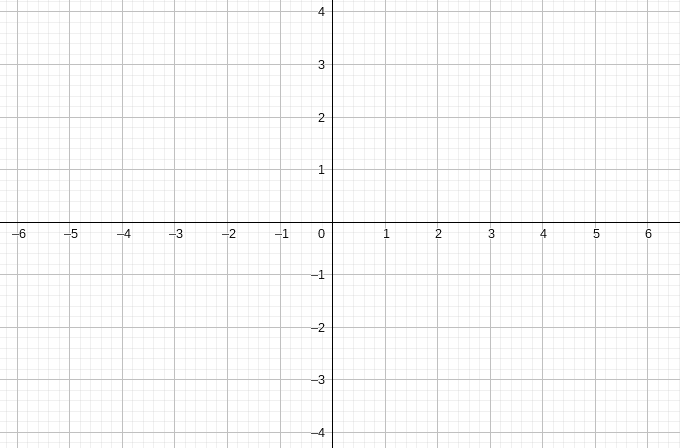
\includegraphics[scale=0.5]{../grid.png}
\end{figure}

\textbf{Conjugados: } Llamamos conjugado de un número complejo $z = a+bi$ a $\bar{z} = a-bi$.

\obs Los conjugados son simétricos respecto del eje $x$.

\subsection{Operaciones en forma binómica} 

\[
[(2+i)+(3-2i) - (-2i)]·[(\rfrac{1}{5}+i)] = ...
\]

\paragraph{División}

Para dividir $z_1 = a+bi$ entre $z_2 = c+di$ hacemos:

\[
\frac{z_1}{z_2} = \frac{a+bi}{c+di} = \frac{a+bi}{c+di} \frac{c-di}{c-di} = \frac{z_1}{z_2}·\frac{\bar{z_2}}{\bar{z_2}}
\]

¿Por qué se multiplica por el conjugado? En la división buscamos $z_? = x+yi$ tal que:

\[\frac{z_1}{z_2} = \frac{a+bi}{c+di} = x+yi\]

Al multiplicar arriba y abajo por el conjugado estamos quitando el número complejo del denominador. De esa manera, operando podemos obtener $x$ e $y$.


\textbf{Ejemplo: }


\paragraph{PRACTICAR CON EL EJERCICIO 8} \hl{Fin de la primera clase}

\subsubsection{Forma polar}

En la representación gráfica de números complejos, podemos utilizar otro sistema de referencia: \textit{módulo} $|z|=r$ y \textit{argumento (ángulo)} $\arg{z} = α$. 
%
Estas son las \concept[Coordenadas polares complejos]{coordenadas polares} y escribimos $z = r_α$

\textbf{Escribe en forma polar:}
\begin{itemize}
	\item $z_1 = 1+i$
	\item $z_2 = 1-i$
	\item $z_3 = 6i$
	\item $z_4 = -2-\sqrt{3}i$
\end{itemize}

\paragraph{Transformación de forma polar a binómica} Dado $z = r_α$, las coordenadas en el plano del número complejo son $(r\cos(α),r\sin(α))$, por lo que podemos escribir:

\[z = \underbrace{r_{α}}_{\text{Polar}} = \underbrace{r·(\cos(α) + i\sin(α))}_{\text{Trigonométrica}} = \underbrace{r\cos(α)}_{a}+\underbrace{r\sin(α)}_{b}i = \underbrace{a+bi}_{\text{Binómica}}\]

\paragraph{Operaciones en forma polar y trigonométrica}

Sean $z_1 = r_α$ y $z_2 = s_β$

$z_1\pm z_2$ necesitamos pasar a forma binómica/trigonométrica. ¿Para qué sirve esta forma entonces? Para multiplicar y dividir, que se hace realmente sencillo 

\hl{Corregir 8ef, 15 abc (solo polar)}. Introducir trigonométrica desde el ejercicio 15.

Operaciones en polar.

\textbf{Multiplicación:} $z_1·z_2 = (r·s)_{α+β} $

\textbf{División:} $\frac{z_1}{z_2} = (\rfrac{r}{s})_{α-β} $

\textbf{Ejemplo}
\[\frac{3_{30}·5_{120}}{\sqrt{15}_{60}·1_{420}}\]


\[\frac{2_{120}·1_{240}}{\sqrt{2}_{60}·2_{30}}\]


\section{Radicación}

Sabemos que $\sqrt{16} = \pm 4$, ¿verdad? Y $\sqrt[4]{16} = \pm 2$, ¿no?

¿Nos habrán mentido desde pequeños sobre esto también? Siento decirte que sí. Vamos a verlo. 

Calcula:
\begin{itemize}
	\item $2^4 = 16$
	\item $(-2)^4 = 16$
	\item $(2i)^4 = 16·i^4 = 16$
	\item $(-2i)^4 = 16·i^4 = 16$ 
\end{itemize}

¡Cuatro raíces! De una manera general $\sqrt[n]{z}$ tiene $n$ soluciones. ¡Vamos a calcularlas! Y para esto es imprescindible la forma polar.

\begin{defn}[Radicación compleja]
$\sqrt[n]{z} = \{s_β\}$ con $s=+\sqrt[n]{|z|}$ y $β=\left\{\displaystyle\frac{\arg(z)+360k}{n}\;\;k\inℕ\right\}$
\end{defn}

\begin{example}
Calcula las 5 raíces de $z=1+i$

\textbf{Solución}
\begin{itemize}
	\item Forma polar: $z=1+i = \sqrt{2}_{45}$
	\item Las raíces serán de la forma $s_β$ con $s=\sqrt[5]{\sqrt{2}}$ y $β=\frac{45+360k}{5}$
	\begin{itemize}
		\item $k=0\to \sqrt[10]{2}_{9}$
		\item $k=1\to \sqrt[10]{2}_{81}$
		\item $k=2\to \sqrt[10]{2}_{153}$
		\item $k=3\to \sqrt[10]{2}_{225}$
		\item $k=4\to \sqrt[10]{2}_{297}$
	\end{itemize}
\end{itemize}
\end{example}



\chapter{Continuidad}



\printindex
\end{document}
\grid
